\documentclass[12pt,a4paper]{report}

\usepackage{float}
\usepackage{graphicx}
\usepackage{fancyhdr}
\usepackage{enumitem}
\usepackage{amsmath}
\usepackage{pgfplots}
\usepackage{datetime}
\usepackage{lastpage}
\usepackage[top=2cm,bottom=2cm,right=2cm,left=2cm]{geometry}

\pgfplotsset{compat=1.18}
\pagestyle{fancy}   
\lhead{Machines and Drives Report}
\rhead{Shawal Mbalire 21/U/0851}
\cfoot{Page~\thepage~of~\pageref{LastPage}}

\begin{document}

\begin{titlepage}
    \begin{center}
        \begin{figure}[H]
            \centering
            
\includegraphics[width=0.5\textwidth]{muk.png}
        \end{figure}

        \vspace{20pt}

        \large COLLEGE OF ENGINEERING, DESIGN, ART AND TECHNOLOGY\\
        \vspace{10pt}
        DEPARTMENT OF ELECTRICAL AND COMPUTER ENGINEERING\\
        \vspace{10pt}
        BACHELOR OF SCIENCE IN ELECTRICAL ENGINEERING\\
        \vspace{10pt}
        SHAWAL MBALIRE\\
        \vspace{10pt}
        21/U/0851\\
        \vspace{20pt}

        \textbf{\Large MACHINES AND DRIVES I LAB REPORT}\\
        \vspace{20pt}

        \begin{table}[h!]
            \centering
            \begin{tabular}{|l|c|l|}
                \hline
                \multicolumn{3}{|c|}{\textbf{GROUP MEMBERS}} \\
                \hline
                \textbf{Name} & \textbf{Program} & \textbf{Registration Number} \\
                \hline
                Shawal Mbalire  & BELE & 21/U/0851 \\
                Namta Dorcus Druscilla & BELE & 22/U/6587 \\
                Kayiwa Philip & BELE & 22/U/6115 \\
                Kigenyi Emmanuel & BELE & 22/U/6140 \\
                Kisaale Kenneth & BELE & 22/U/6161 \\
                Muadi Kassim Ismail & BELE & 22/U/3383/PSA \\
                Mwanje Umar & BELE & 22/U/6443 \\
                Nsumba Vicent & BELE & 22/U/6730 \\
                Nuwamanya Pancras & BELE & 22/U/6746 \\
                Odong Ivan Joe & BELE & 22/U/21259/PSA \\
                Onyait Richard & BELE & 22/U/21263/PS \\
                Ssebadduka Marvin & BELE & 22/U/6889 \\
                Swalik Natumanya & BELE & 22/U/6688 \\
                Kyeyune Jordie & BELE & 20/U/0449 \\
                Mukisa Joshua & BELE & 22/U/6367 \\
                Kigozi Stuart James & BELE & 22/U/21224/PSA \\
                Yiga Hakim & BELE & 22/U/3966/PSA \\
                \hline
            \end{tabular}
        \end{table}
       
        \vspace{20pt}

        \normalsize Instructor: Mr. Robinson Ntege\\
        \vspace{10pt}

        \normalsize \today
        \vspace{20pt}

    \end{center}
\end{titlepage}

\tableofcontents
\newpage

\listoffigures
\newpage

\listoftables
\newpage


\chapter{Experiment to Determine the Transformation Ratio and the Equivalent Circuit Parameters of a Single-Phase Transformer}

\section{Objectives}
The objectives of this experiment are as follows:
\begin{enumerate}[label=\roman*.]
    \item \textbf{To determine the transformation ratio, \(k\):} The transformation ratio of a transformer, typically denoted by \(k\), is the ratio of the primary voltage to the secondary voltage (or vice versa) under no-load conditions. This ratio is crucial as it helps determine the efficiency of voltage transformation between primary and secondary windings. For an ideal transformer, \(k\) is equal to the turns ratio between the primary and secondary windings.
    
    \item \textbf{To determine the equivalent circuit parameters:} The equivalent circuit of a transformer is used to represent its internal impedance, losses, and magnetizing characteristics in a simplified form. By finding these parameters, we can approximate the performance characteristics, including voltage regulation and efficiency, of the transformer under load conditions. This includes components such as winding resistances, leakage reactances, and magnetizing impedance.
\end{enumerate}

\section{List of Apparatus}
The following apparatus were used to conduct the experiment:
\begin{enumerate}[label=\roman*.]
    \item \textbf{Single-phase transformer:} The core component of the experiment, this transformer has primary and secondary windings that enable voltage transformation. The transformer chosen is rated to match the experiment's voltage requirements.
    
    \item \textbf{Variac:} A variac, or variable AC transformer, is used to gradually increase or decrease the input voltage to the transformer in a controlled manner. It helps in safely applying and adjusting voltage levels for measurements without causing sudden changes that could damage the equipment.
    
    \item \textbf{AC ammeters and voltmeters:} These are used to measure the AC current and voltage at the primary and secondary sides of the transformer. They are essential for obtaining accurate measurements of the transformation ratio and equivalent circuit parameters.
    
    \item \textbf{Wattmeter:} A wattmeter measures the real power consumed by the transformer. This is particularly useful for determining the core losses and copper losses in the transformer, which are necessary for calculating the equivalent circuit parameters.
\end{enumerate}

\section{Theory}
The performance and characteristics of a single-phase transformer can be analyzed using an equivalent circuit model. This model simplifies the transformer’s behavior into a series of components that represent its various internal losses and impedance. By conducting specific tests, we can determine the values of these parameters, which provide insights into the transformer’s efficiency, voltage regulation, and other operational characteristics.

In the equivalent circuit model shown in Figure~\ref{fig_1}, the parameters are defined as follows:
\begin{itemize}
    \item \textbf{\( r_0 \) and \( x_0 \)}: These represent the core loss components, which include hysteresis and eddy current losses. These parameters are derived from the no-load or open circuit test, where the secondary winding is left open, and a small voltage is applied to the primary winding. During this test, the core losses dominate, as there is minimal current in the winding, allowing us to isolate these parameters.

    \item \textbf{\( r_1 \) and \( x_1 \)}: These parameters represent the equivalent series resistance and leakage reactance of the transformer windings. They are primarily determined through the short-circuit test, where the secondary winding is shorted and a reduced voltage is applied to the primary winding until rated current flows. This test is conducted under conditions where the winding losses dominate, enabling the calculation of \( r_1 \) and \( x_1 \).

    \item \textbf{Open Circuit Test}: The open circuit test is performed by applying the rated voltage to the primary winding with the secondary side left open. This allows for measurement of the core losses and helps us find \( r_0 \) and \( x_0 \), which correspond to the core resistance and reactance.

    \item \textbf{Short Circuit Test}: The short circuit test is conducted by shorting the secondary winding and applying a reduced voltage to the primary winding. This test helps measure the copper losses (due to winding resistance) and leakage reactances, allowing us to determine \( r_1 \) and \( x_1 \) accurately.

\end{itemize}

\begin{figure}[H]
    \centering
    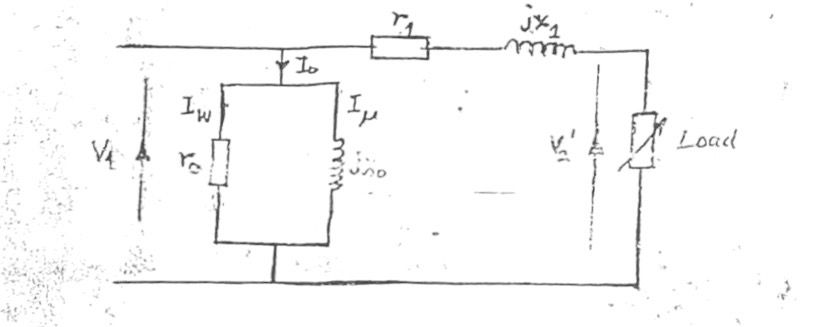
\includegraphics[width=0.8\linewidth]{figure_1_1.jpeg}
    \caption{Single-phase transformer equivalent circuit}
    \label{fig_1}
\end{figure}

The equivalent circuit provides a way to predict the transformer’s voltage regulation and efficiency under various load conditions. By using the open circuit and short circuit test results, we can calculate these parameters, which help us model and understand the performance characteristics of the transformer in practical applications.

\section{Procedures}

\subsection{Ratio Test}
This test is conducted to determine the transformation ratio \( k \) of the transformer. The transformation ratio is the ratio of the primary voltage to the secondary voltage and is fundamental in assessing the transformer's ability to convert voltages.

\begin{enumerate}
    \item Connect the circuit as shown in Figure~\ref{fig_2} below, with the variac connected to the primary side of the transformer to control the input voltage.
    
    \begin{figure}[H]
        \centering
        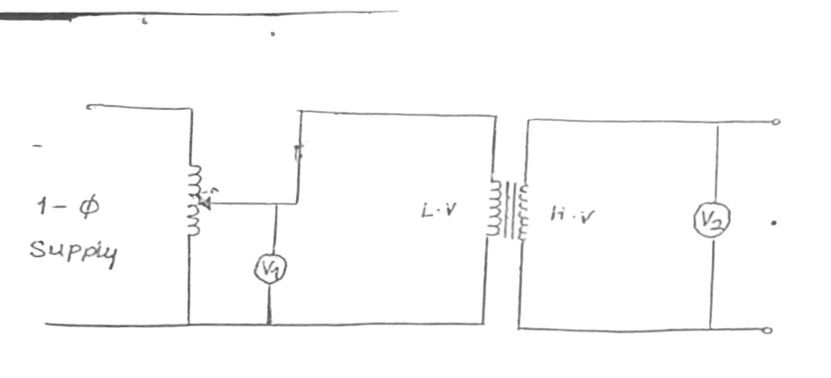
\includegraphics[width=0.8\linewidth]{figure_2_2.jpeg}
        \caption{Single-phase transformer ratio test setup}
        \label{fig_2}
    \end{figure}
    
    \item Vary the output of the variac from 30V to 90V in steps of 10V, allowing for multiple data points to better assess the transformation ratio across a range of input voltages.
    
    \item Measure and record the voltage on the low voltage (LV) and high voltage (HV) sides of the transformer using accurate AC voltmeters. This data will provide the basis for calculating the transformation ratio.
    
    \item Calculate \( k = V_2 / V_1 \) for each voltage step to determine the transformation ratio at various levels. Record these values as shown in the table below.

\end{enumerate}

\begin{table}[H]
    \centering
    \caption{Power Measurements and Ratios}
    \begin{tabular}{|c|c|c|c|}
    \hline
    $V_1 (\text{V})$ & $W_{\text{input}} (\text{W})$ & $W_{\text{output}} (\text{W})$ & $\eta = \frac{W_{\text{output}}}{W_{\text{input}}}$ \\ \hline
    30 & 62  & 2.07 \\ \hline
    40 & 81  & 2.03 \\ \hline
    50 & 107 & 2.14 \\ \hline
    60 & 126 & 2.10 \\ \hline
    70 & 146 & 2.08 \\ \hline
    80 & 164 & 2.05 \\ \hline
    90 & 180 & 2.00 \\ \hline
    \end{tabular}
    \end{table}
    

The variation in \( k \) across the voltage range provides insights into the transformer's performance and potential deviations from ideal behavior due to internal losses or non-linearities in the magnetic core.

\subsection{Open Circuit Test}
The open circuit test is conducted to determine the core loss parameters of the transformer, which include hysteresis and eddy current losses. These losses are inherent in the magnetic core and are dependent on the applied voltage and frequency.

\begin{enumerate}
    \item Make the necessary connections as shown in Figure~\ref{fig_3}, ensuring the high voltage (HV) side of the transformer is left open while the low voltage (LV) side is connected to the variac.

    \begin{figure}[H]
        \centering
        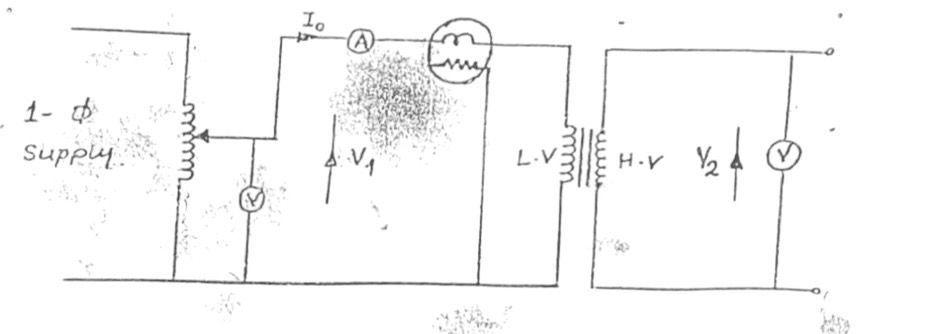
\includegraphics[width=0.8\linewidth]{figure_3_3.jpeg}
        \caption{Single-phase transformer open circuit test setup}
        \label{fig_3}
    \end{figure}

    \item Apply a gradually increasing voltage at the LV side using the variac, taking care to increase the voltage to the rated voltage of the transformer. This helps ensure that the test simulates real operating conditions and yields accurate core loss values.
    
    \item Measure and record the power input \( P_0 \), current \( I_0 \), and voltage \( V_2 \) at the LV and HV sides respectively. The power input \( P_0 \) measured by the wattmeter represents the core losses.
    
    \item Repeat the procedure at different input voltage levels to observe the effect of voltage variation on core losses and magnetizing current. Record these readings as shown in the table below.

    \begin{table}[H]
        \centering
        \caption{Voltage, Current, Power, and Efficiency Measurements}
        \begin{tabular}{|c|c|c|c|c|}
        \hline
        $V_1$ (V) & $I_0$ (A) & $P_0$ (W) & $n_2$ (rpm) & $\Phi_0 = \frac{P_0}{V_1 I_0}$ \\ \hline
        30        & 0         & 0         & 66          & 0.000                          \\ \hline
        40        & 0         & 0         & 78          & 0.000                          \\ \hline
        50        & 5         & 0.5       & 101         & 0.200                          \\ \hline
        60        & 10        & 1.6       & 124         & 0.104                          \\ \hline
        \end{tabular}
        \end{table}
        

    \item Determine the open circuit parameters \( r_0 \) and \( x_0 \) based on the measurements recorded in the table above. The values of \( r_0 \) and \( x_0 \) provide insights into the core losses and magnetizing reactance, which are essential components of the equivalent circuit.
    
    \textbf{\textit{The open circuit parameters are calculated using the recorded data and are presented in the table above.}}
\end{enumerate}

\subsection{Short Circuit Test}
The short circuit test is conducted to determine the winding resistance (\( r_1 \)) and leakage reactance (\( x_1 \)) of the transformer. These parameters are crucial in assessing the transformer’s impedance under load and help predict its performance under rated conditions.

\begin{enumerate}
    \item Connect the transformer as shown in Figure~\ref{fig_4}, with the low voltage (LV) side short-circuited. Ensure that all connections are secure to avoid any unsafe conditions.

    \begin{figure}[H]
        \centering
        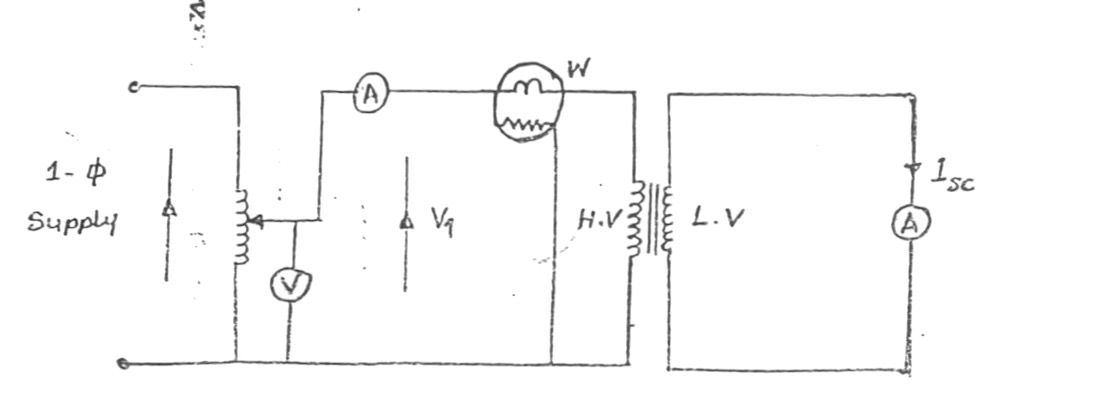
\includegraphics[width=0.8\linewidth]{figure_4_4.jpeg}
        \caption{Short circuit test setup for single-phase transformer}
        \label{fig_4}
    \end{figure}
    
    \item Gradually apply a small input voltage \( V_{1} \) on the high voltage (HV) side of the transformer using a variac until the rated current flows through the LV winding. It is important to limit the applied voltage to approximately 5-10\% of the transformer's rated voltage, as this is sufficient to produce the rated current without risking core saturation or damage.
    
    \item Measure and record the power input \( P_{SC} \), the corresponding current \( I \), and the power factor on the HV side. The power input \( P_{SC} \) represents the copper losses in the transformer windings under short-circuit conditions, allowing for the calculation of equivalent winding resistance.
    
    \item Ensure that the input voltage does not exceed approximately 8\% of the rated HV voltage to avoid overheating and maintain test accuracy.
    
    \item Repeat the procedure for lower values of short circuit currents \( I_{SC} \) by adjusting the input voltage. This allows for multiple data points to observe how the current and power losses vary with changes in voltage and current levels.
    
    \item Record the results in the table below for analysis.

    \begin{table}[H]
        \centering
        \caption{Voltage, Current, Power, and Efficiency Measurements}
        \begin{tabular}{|c|c|c|c|c|}
        \hline
        $V_1$ (V) & $I_a$ (A) & $P_a$ (W) & $R$ ($\Omega$) & $\Phi = \frac{P_a}{V_1 I_a}$ \\ \hline
        2         & 0         & 1.6       & 1.8            & 0.000                          \\ \hline
        4         & 10        & 9.0       & 4.7            & 0.532                          \\ \hline
        6         & 25        & 13.2      & 6.6            & 0.631                          \\ \hline
        8         & 40        & 14.5      & 8.2            & 0.610                          \\ \hline
        10        & 65        & 19.0      & 10.2           & 0.637                          \\ \hline
        12        & 90        & 22.5      & 12.9           & 0.581                          \\ \hline
        14        & 115       & 26.5      & 14.8           & 0.555                          \\ \hline
        16        & 150       & 30.5      & 16.5           & 0.568                          \\ \hline
        18        & 195       & 35.0      & 18.5           & 0.586                          \\ \hline
        20        & 230       & 38.5      & 20.2           & 0.569                          \\ \hline
        \end{tabular}
        \end{table}
        

    \item Comment on your results. Analyze the results to determine the short-circuit parameters of the transformer, specifically the equivalent series resistance \( r_1 \) and leakage reactance \( x_1 \), using the measured power and current values.

    \textbf{\textit{Observations:}} For small variations in voltage, there is a significant increase in current, indicating the low impedance of the windings under short-circuit conditions. The increasing power factor values show the relationship between the applied voltage and the resulting short-circuit current. These values are crucial for estimating the internal losses and impedance of the transformer.
    
    \textbf{\textit{The short-circuit parameters are calculated from the recorded data and are presented in the table above.}}
    \section{Calculation of  K}

The K value of the data points \( 2.07, 2.03, 2.14, 2.10, 2.08, 2.05, 2.00 \) is calculated as:

\[
\text{K} = \frac{2.07 + 2.03 + 2.14 + 2.10 + 2.08 + 2.05 + 2.00}{7} = \frac{14.47}{7} \approx 2.07
\]

Thus, the average value is approximately \( 2.07 \).

    \section{Open Circuit Parameters}

\begin{enumerate}
    \item \textbf{Core loss resistance referring to the LV side:}
    \begin{equation}
        R_{c(\text{LV})} = \frac{V_1^2}{P_0} = 360 \ \Omega
    \end{equation}

    \item \textbf{Core loss resistance referring to the HV side:}
    \begin{equation}
        R_{c(\text{HV})} = \left( \frac{N_2}{N_1} \right)^2 R_{c(\text{LV})} = 1440 \ \Omega
    \end{equation}

    \item \textbf{Magnetizing reactance referring to the LV side:}
    \begin{equation}
        X_{m(\text{LV})} = \frac{V_1}{\sqrt{I_0^2 - \left( \frac{P_0}{V_1} \right)^2}} = 37.705 \ \Omega
    \end{equation}

    \item \textbf{Magnetizing reactance referring to the HV side:}
    \begin{equation}
        X_{m(\text{HV})} = \left( \frac{N_2}{N_1} \right)^2 X_{m(\text{LV})} = 150.82 \ \Omega
    \end{equation}
\end{enumerate}

    \section{Short Circuit Parameters}

\begin{enumerate}
    \item \textbf{Core loss resistance referring to the LV side:} 
    \begin{equation}
        R_{c(\text{LV})} = \frac{V_1^2}{P_c} = 1.739 \ \Omega
    \end{equation}

    \item \textbf{Core loss resistance referring to the HV side:}
    \begin{equation}
        R_{c(\text{HV})} = \left( \frac{N_2}{N_1} \right)^2 R_{c(\text{LV})} = 6.957 \ \Omega
    \end{equation}

    \item \textbf{Magnetizing reactance referring to the LV side:}
    \begin{equation}
        X_{m(\text{LV})} = \frac{V_1^2}{I_0^2 - \left( \frac{P_0}{V_1} \right)^2} = 1.204 \ \Omega
    \end{equation}

    \item \textbf{Magnetizing reactance referring to the HV side:}
    \begin{equation}
        X_{m(\text{HV})} = \left( \frac{N_2}{N_1} \right)^2 X_{m(\text{LV})} = 4.817 \ \Omega
    \end{equation}
\end{enumerate}

\end{enumerate}


\chapter{Experiment to determine parameters and performance characteristics of Induction Motors.}
\section{Objectives}
\begin{enumerate}
    \item To determine the equivalent circuit parameters of the induction motor, including stator resistance, rotor resistance, and magnetizing reactance, by conducting no-load, blocked rotor, and load tests. These parameters provide insights into the electrical behavior of the motor and are essential for modeling its performance.
    \item To predict the performance characteristics of the motor, such as torque, efficiency, and power factor, across different load conditions. This will involve using the equivalent circuit parameters derived from the tests to calculate expected motor behaviors and comparing these with experimental results to understand the motor's efficiency and suitability for various applications.
\end{enumerate}

\section{List of Apparatus}
\begin{enumerate}
    \item \textbf{Power Supply (mod AV -1/V)}: Provides a stable and adjustable AC voltage source for powering the induction motor. This allows control over the voltage applied to the motor during no-load, blocked rotor, and load tests.
    
    \item \textbf{4 Variable Resistors (RC3-PT)}: Used to vary the resistance in the circuit, helping to simulate different load conditions on the motor during testing. This allows for control of current flow and the testing of motor response under varying loads.
    
    \item \textbf{Multifunctional Digital Instrument (AZ VIP 10/EV)}: Measures voltage, current, power, and power factor, providing accurate electrical parameter readings essential for calculating the motor’s equivalent circuit parameters and evaluating efficiency and performance.
    
    \item \textbf{Digital Torque and Speed Measurement Unit (Um-G1/EV)}: Measures the torque output and rotational speed of the motor, critical for determining the motor’s performance characteristics such as torque-speed relationship and efficiency.
    
    \item \textbf{3-Phase Induction Motor (mod P-4/EV)}: The main subject of the experiment, this motor will undergo various tests (no-load, blocked rotor, and load tests) to determine its electrical and performance characteristics, allowing for equivalent circuit modeling and performance analysis.
\end{enumerate}

\section{Theory}
Induction motors are widely used for their simplicity, reliability, and efficiency in various industrial applications. They operate by creating a rotating magnetic field in the stator windings, which induces a current in the rotor. This interaction generates a torque on the rotor, causing it to turn. However, the performance of an induction motor depends on several key parameters, which can be determined through specific tests and measurements.

The equivalent circuit of an induction motor represents its electrical behavior and includes the following key components:
\begin{itemize}
    \item \textbf{Stator resistance} ($R_1$) and \textbf{stator leakage reactance} ($X_1$): Represent the resistance and reactance of the stator windings, which cause energy losses and affect the motor’s efficiency.
    \item \textbf{Rotor resistance} ($R_2$) and \textbf{rotor leakage reactance} ($X_2$): Represent the resistance and reactance of the rotor windings, which contribute to energy losses, and are influenced by the slip of the motor.
    \item \textbf{Magnetizing reactance} ($X_m$): Represents the reactance of the motor’s magnetic field, which links the stator and rotor. This parameter is crucial for determining the motor's magnetizing current and overall efficiency.
\end{itemize}

To accurately model the motor's performance, these parameters are determined through three common tests: the no-load test, the blocked rotor test, and the load test.

\subsection{Tests for Determining Motor Parameters}

\begin{itemize}
    \item \textbf{No-Load Test}: Conducted by running the motor with no mechanical load applied to the rotor. This test measures the magnetizing current, which is responsible for producing the magnetic field in the motor, and the rotational losses. It helps determine the magnetizing reactance ($X_m$) and core losses.
    
    \item \textbf{Blocked Rotor Test}: In this test, the rotor is physically blocked from rotating, and the stator is supplied with a low voltage to produce the rated current. This test helps to determine the stator and rotor resistance ($R_1$, $R_2$) as well as the leakage reactances ($X_1$, $X_2$) by simulating the locked-rotor conditions, which occur when the motor starts or under heavy load conditions.
    
    \item \textbf{Load Test}: This test applies a known mechanical load to the motor and measures the motor’s output torque, speed, current, voltage, and power factor. It provides practical data to evaluate the motor’s efficiency, torque-speed performance, and power factor under normal operating conditions.
\end{itemize}

\subsection{Equivalent Circuit Model}
Once the parameters from these tests are obtained, they can be used to build an equivalent circuit model of the motor. The equivalent circuit is a simplified representation of the motor’s electrical behavior, which includes the following components:
\begin{itemize}
    \item \textbf{Stator resistance} ($R_1$) and \textbf{stator leakage reactance} ($X_1$) in series.
    \item \textbf{Rotor resistance} ($R_2$) and \textbf{rotor leakage reactance} ($X_2$) in parallel with the magnetizing reactance ($X_m$).
    \item The mechanical power developed by the motor can be calculated using the torque and rotational speed data obtained from the load test, helping to evaluate the motor’s efficiency.
\end{itemize}

The equivalent circuit model allows engineers to predict the motor's performance in various operating conditions by calculating the efficiency, slip, and torque characteristics. This model is crucial for optimizing motor design, selection, and operation in specific applications, ensuring that motors perform efficiently under varying loads.

\section{Procedure}

\subsection{Light Running Test}
\begin{enumerate}
    \item Connect the machine as shown in the figure below.
    \begin{figure}[H]
        \centering
        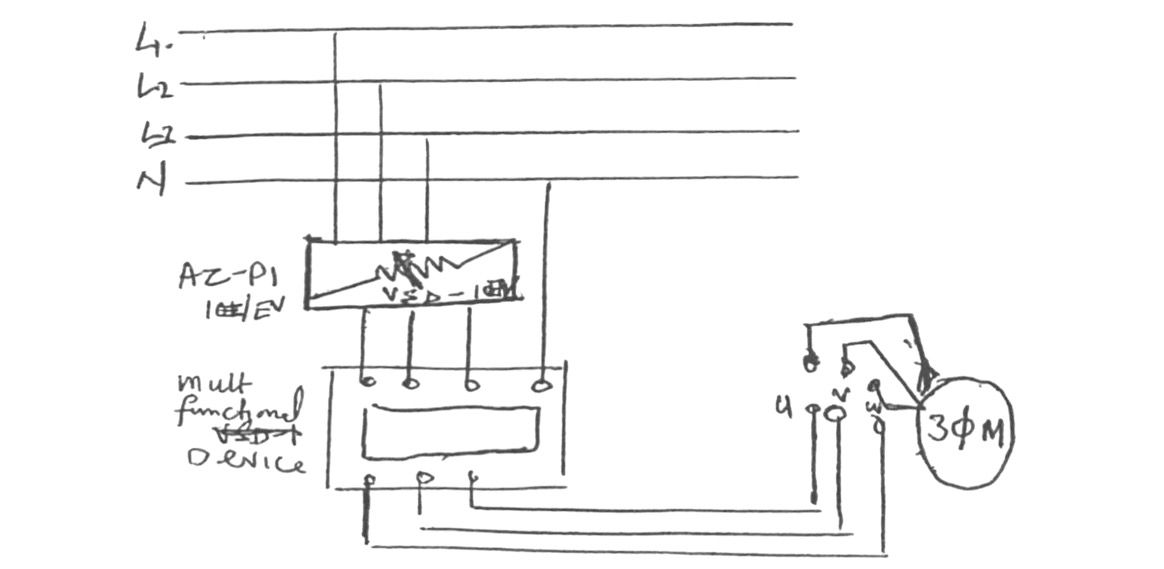
\includegraphics[width=\linewidth]{figure_5_5.jpeg}
        \caption{Light running test: without load}
        \label{fig_5}
    \end{figure}
    \item Start the motor by applying normal frequency, reduced voltage, and gradually increase the input voltage to its rated value.
    \item Note down the readings for voltage, current, power, and speed at different voltages.
    \item The results are tabulated below.

\begin{table}[H]
    \centering
    \caption{Table of Results with Calculations}
    \begin{tabular}{|c|c|c|c|c|c|c|}
    \hline
    \(\text{V (V)}\) & \(\text{I (A)}\) & \(\text{W}_1 (\text{W})\) & \(\text{W}_2 (\text{W})\) & \(\text{W}_3 (\text{W})\) & n(rpm) & \(\rho = \frac{W_1 - W_2}{W_1}\) \\ \hline
    30  & 0.612  & 4.6  & 4.5  & 5.8  & 0    & 0.0217   \\ \hline
    40  & 0.920  & 10.2 & 10.2 & 11.2 & 0    & 0.00005  \\ \hline
    50  & 1.254  & 19.2 & 19.6 & 21.4 & 33   & -0.0209  \\ \hline
    60  & 1.550  & 29.9 & 30.1 & 33.3 & 42   & -0.00677 \\ \hline
    70  & 1.880  & 44.5 & 45.9 & 49.1 & 288  & -0.0316  \\ \hline
    80  & 0.925  & 33.9 & 34.1 & 36.2 & 2648 & -0.00599 \\ \hline
    90  & 0.608  & 27.1 & 28.3 & 31.7 & 2765 & -0.0443  \\ \hline
    100 & 0.533  & 26.1 & 27.4 & 30.1 & 2812 & -0.0498  \\ \hline
    110 & 0.488  & 26.2 & 26.5 & 29.6 & 2837 & -0.0115  \\ \hline
    \end{tabular}
    \end{table}
    
    \item Plot Voltage ($V$) against Speed ($n$).
\end{enumerate}

\begin{tikzpicture}
    \begin{axis}[
        compat=1.18,
        width=\linewidth, % Use the full width
        xlabel = $n(rpm)$,
        ylabel = $V(V)$,
        xtick = {0, 89, 320, 2601, 2779, 2839, 2869}, % Customize x-axis ticks to avoid overlap
        xticklabel style={rotate=45}, % Rotate labels for better fit
    ]
    \addplot [
        table/row sep=\\,
        mark=*,
        color=blue,
    ]
    table {
        n     V  \\
        0     30 \\
        0     40 \\
        0     50 \\
        89    60 \\
        320   70 \\
        2601  80 \\
        2779  90 \\
        2839  100 \\
        2869  110 \\
    };
    \end{axis}
\end{tikzpicture}

\subsection{Blocked Rotor Test}
\begin{enumerate}
    \item The connection is set up as shown below. Block the rotor with a load cell.
    \begin{figure}[H]
        \centering
        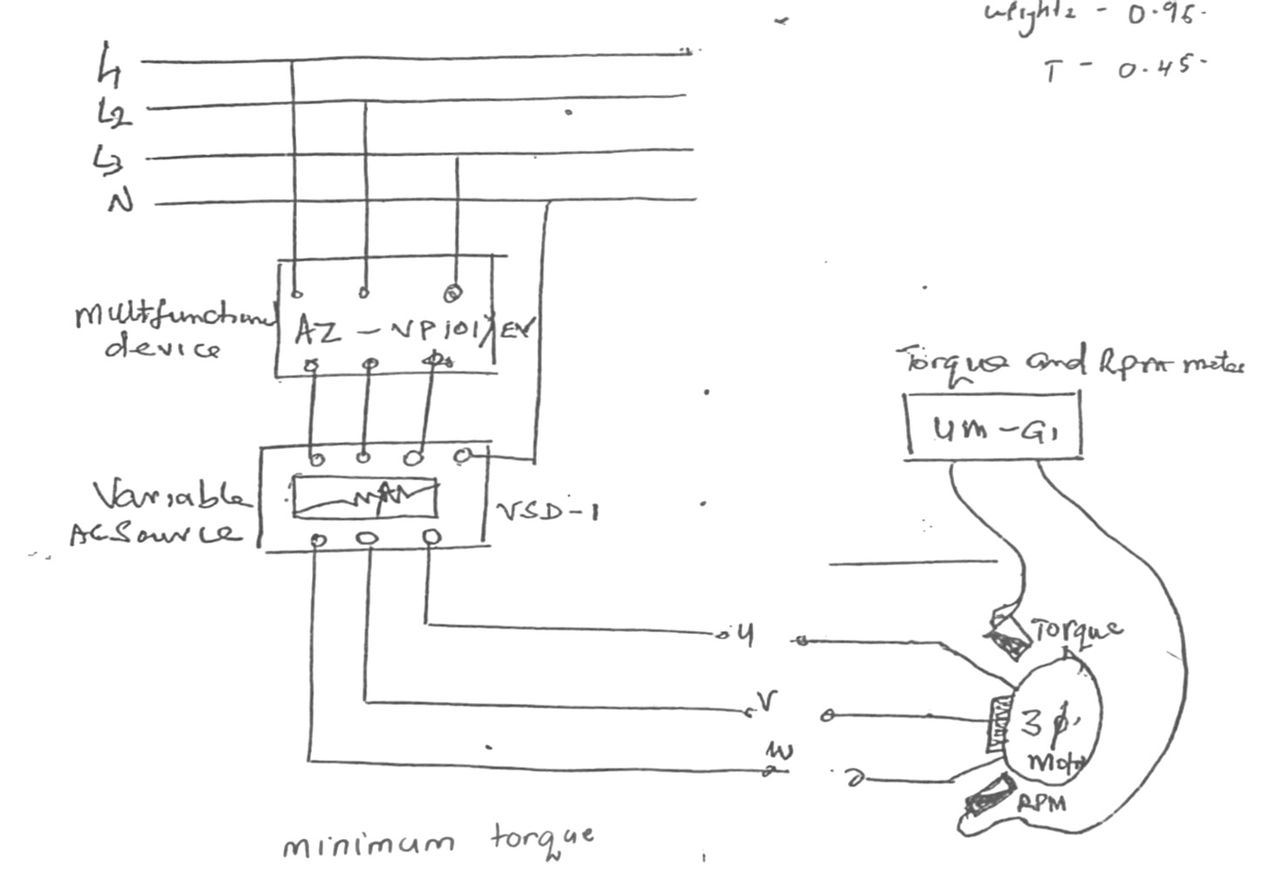
\includegraphics[width=\linewidth]{figure_6_6.jpeg}
        \caption{Blocked rotor}
        \label{fig_6}
    \end{figure}
    \item Measure:
    We determined the open circuit parameters of the machine under steady-state conditions as follows:

The open circuit voltage was calculated as:
\[
V_{\text{oc}} = 90 \, \text{V} \quad \text{and} \quad I_{\text{oc}} = 90 \, \text{A}
\]
The line voltage is:
\[
V_{\text{L}} = \sqrt{3} \times V_{\text{oc}} = \sqrt{3} \times 51.96 = 90 \, \text{V}
\]

The no-load power is:
\[
P_0 = P_1 + P_2 + P_3 = 27.1 \, \text{W} + 28.3 \, \text{W} + 31.7 \, \text{W} = 87.1 \, \text{W}
\]

Now, we calculate the core loss resistance:
\[
R_{\text{core}} = \frac{V}{I} = \frac{90}{0.608} = 85.461 \, \Omega
\]

Next, the magnetizing reactance:
\[
X_{\text{m}} = \frac{3 \times V_{\text{oc}}}{2} = \frac{3 \times 0.608}{2} = 77.062 \, \Omega
\]

Finally, we calculate the total magnetizing reactance:
\[
X_{\text{m total}} = \sqrt{R_{\text{core}}^2 - X_{\text{m}}^2} = \sqrt{85.461^2 - 77.062^2} = 36.946 \, \Omega
\]
\end{enumerate}

\chapter{Errors}

In conducting practical tests on transformers and induction motors, various sources of errors can affect the accuracy of measurements and results. Key sources of errors in transformer and motor testing include:

\section{Sources of Errors}

\begin{enumerate}
    \item \textbf{Instrument Accuracy}: Inaccuracies in voltmeters, ammeters, and wattmeters can lead to measurement errors during open and short circuit tests.
    \item \textbf{Connection Errors}: Poor connections or loose terminals can cause significant deviations in test results, especially during the high-current blocked rotor test.
    \item \textbf{Temperature Effects}: Changes in winding resistance due to temperature variations can affect results in short circuit and blocked rotor tests.
\end{enumerate}

\section{Error Minimization}

To minimize errors during the experiments, the following steps should be taken:

\begin{enumerate}
    \item \textbf{Instrument Calibration}: Ensure all measuring instruments are calibrated before testing to reduce reading errors.
    \item \textbf{Secure Connections}: Tighten all connections securely to avoid contact resistance that could affect results.
    \item \textbf{Temperature Control}: Conduct tests at stable temperatures or record temperature data to account for changes in resistance.
\end{enumerate}

\chapter{Conclusion}

The practical lab sessions on transformer and induction motor testing provided a solid foundation for understanding core principles of machine characteristics. By performing open and short circuit tests on transformers, we were able to accurately determine parameters like the equivalent impedance and transformer ratio. The light running and blocked rotor tests on induction motors allowed us to determine their key characteristics, such as slip and torque, under different operating conditions.

Overall, the experiments highlighted the importance of accurate measurement techniques, error minimization, and methodical setup for obtaining reliable data on machine performance. These hands-on exercises are crucial for developing practical skills in electrical machine testing and diagnostics.

\nocite{*}            
\bibliographystyle{ieeetr}  
\bibliography{ref} 


\end{document}